\addtocontents{toc}{\protect\setcounter{tocdepth}{0}}

\section{Introduction}



LLMs have proved to be powerful copilots in scientific research~\citep{AI4Science2023TheIO}, demonstrating their great potential for accelerating scientific discovery.
Despite the promising finding, a more ambitious question remains: \textit{Can we simulate the human research community with LLMs}? Answering such a question has multiple benefits: (1) simulating the human research community helps understand the underlying process behind the discovery of existing research ideas; (2) it can further help democratize and accelerate the discovery process of new research ideas.

However, simulating the human research community is challenging, as it involves leveraging multiple LLM agents to interact with complex research data. While existing multi-agent LLM frameworks have been successfully applied to areas like social simulation~\citep{zhou2023sotopia,Gao2023S3SS} and game simulation~\citep{hua2023war,xu2023language}, they are not well-suited for simulating research communities due to the complexity of collaborative research activities like paper writing and review writing. Although recent efforts have explored research automation using LLMs, these frameworks are typically limited to specific research tasks, such as idea generation~\citep{girotra2023ideas, baek2024researchagent} or code experimentation~\citep{huang2024mlagentbench}, or focus on simulating single-agent workflows~\citep{lu2024ai}. These frameworks cannot simulate collaborative research activities where researchers with diverse backgrounds work together to brainstorm ideas, review papers, etc—processes that are fundamental to modern human research.

\begin{figure*}[t]
    \centering
    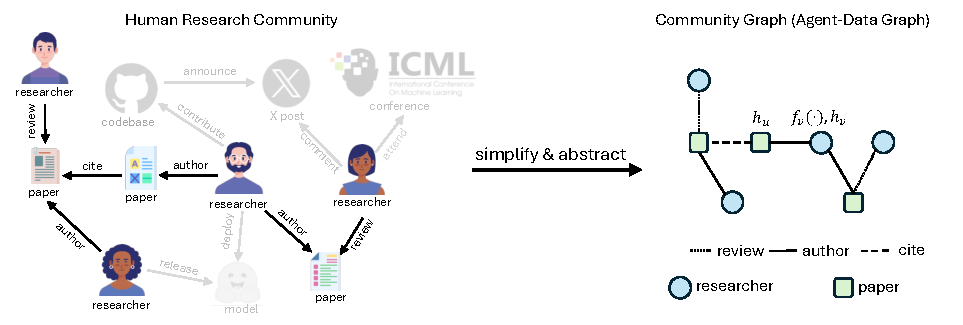
\includegraphics[width=0.88\linewidth]{./figs/community_graph_definition.pdf}
    \caption{\textbf{Abstracting and simplifying human research community as an agent-data graph, \ie, community graph}. An agent-data graph has researchers as agent nodes and blogs, codebases, and papers as data nodes. Without losing generality, we abstract it into a simplified version with only researcher and paper nodes and focus on critical research tasks, including paper reading, paper writing, and review writing. Each data node has a hidden state $h_u$, and each agent node is paired with an agent function $f_v(\cdot)$ and a hidden state $h_v$.}
    \label{fig:community-graph}
    \vspace{-4mm}
\end{figure*}

\xhdr{Research community as graph}
Our key observation is that the deeply interconnected research community can be naturally represented as graphs. Indeed, similar graph structures like citation networks~\citep{newman2001structure} and academic social networks~\citep{Tang2008ArnetMinerEA} have been extensively studied within data mining research, with proven values in applications such as citation prediction~\citep{holm2020longitudinal}, recommendation~\citep{West2016ARS}, and community detection~\citep{Yang2012DefiningAE}.
However, introducing LLMs to a graph-structured research community can extend these previous works from prediction and analysis with existing data to dynamic simulation and real-time forecasting.

\xhdr{Novel framework for research simulation}
In this work, we propose \envname, a simulator of the human research community. To bridge the gap between existing multi-agent simulation frameworks and the complexity of research activities, we propose a graph-based framework, inspired by the message-passing mechanism in Graph Neural Networks (GNNs), for multi-agent simulation.
Concretely, as shown in Figure \ref{fig:community-graph}, we propose a new concept of \textit{agent-data graph} with 2 generic types of nodes: (1) \textit{agent} nodes, suitable for entities like agents; (2) \textit{data} nodes, suitable for entities such as papers, reviews, and blogs. 
Agent-data graphs are unique from standard heterogeneous graphs; here, the key conceptual difference between agent and data nodes is that an agent node can be considered a function over data nodes.
To inference on agent-data graphs, we propose a \textit{TextGNN} framework where message-passing processes are defined based on text-form information processing with LLMs, thanks to their strong in-context learning~\citep{wei2023larger} and reasoning~\citep{lee2024reasoning} ability. 
We apply the proposed agent-data graph and TextGNN to the research simulation. Here, a research community can be regarded as a special form of agent-data graph, called \textit{community graph}, with research agents and research papers as two types of nodes, and we consider three types of edges (review, author, and cite) in the graph. Different community activities, such as paper writing and review writing, can be modeled as special message-passing processes on the community graph.




\xhdr{Novel evaluation for research simulation} 
With \envname for research simulation, a further research question is to evaluate the quality of that. Prior works primarily use human evaluation with breakdown metrics such as novelty, excitement, feasibility, and expected effectiveness~\citep{si2024can,hu2024nova}. These approaches inevitably suffer from subjectiveness and high costs. In our work, since \envname functions as a simulator, our primary focus is on measuring how closely its outputs align with those of the real-world research community. Community graphs naturally provide a similarity-based evaluation method by masking a given paper node in the community graph and evaluating whether a simulator can reconstruct the masked nodes. This definition focuses on simulation similarity, making it scalable and objective. Based on such a node masking prediction task, we build a benchmark called \benchname with 1,000 paper writing tasks and 200 review writing tasks requiring multi-agent collaboration.


\xhdr{Main discoveries} Based on the evaluation results from \benchname, we highlight three key findings: (1) \envname effectively simulates collaborative research activities, achieving an average similarity score of 0.68 for paper writing and 0.49 for review writing, as measured by the state-of-the-art text embedding model; (2) \envname demonstrates robustness and effectiveness in research simulation, showing improvement when more agents are added and maintaining performance when including unrelated papers; (3) \envname inspires interdisciplinary research, generating innovative ideas that combine insights from NLP, criminology, and astronomy and does not exist in the real-world research.


\xhdr{Stressing ethical concerns} As our work targets simulating the human research community, multiple ethical concerns, including facilitating research plagiarism and producing low-quality or misleading claims, appear. These ethical concerns are addressed in detail in Appendix~\S\ref{appendix:ethical}.

